\section{Methodologies}
    \subsection{Preprocessing}
        \paragraph{}
        An MFCC is a 2-D array. One dimension represents time while the other dimension represents the different frequencies. By analyzing the .json file created from the save\_mfcc method, we can observe the following. There are 9986 mfccs in total where each mfcc is mapped to a specific music genre. A genre is labelled as an integer from 0 to 9 because there are 10 different genres in our dataset (i.e. ['pop', 'metal', 'disco', 'blues', 'reggae', 'classical', 'rock', 'hiphop', 'country', 'jazz']). 
        
        Also, by looking at the distribution of our genres, we can see that it is evenly distributed. This is because the dataset contains 100 sample songs for each music genre. Note that, one song was removed in the jazz genre as jazz0054.wav was corrupted and could not be read. We can observed the genre distribution through our plot\_histogram function.
           \begin{figure}[H]
        \centering
        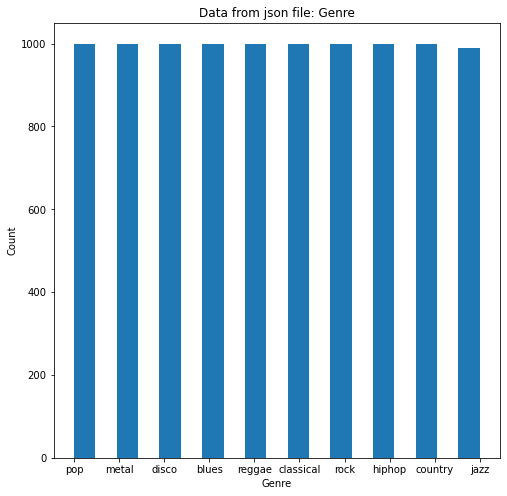
\includegraphics[width=0.35\textwidth]{images/genre.png} 
        \caption{Distribution of music genre data}
    \end{figure}
        
        \paragraph{}
        Also, the visual representation of each genre through a spectrogram which shows how quickly the frequencies themselves are changing over time. The first axis is frequency while the second axis is time. 
        
          \begin{figure}[H]
        \centering
        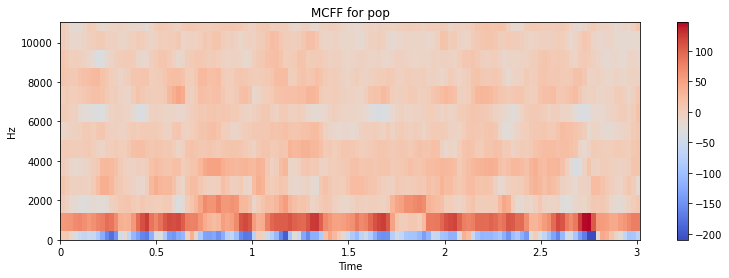
\includegraphics[width=0.5\textwidth]{images/pop_mfcc.png} 
        \caption{MFCC example}
        \end{figure}
        
    \subsection{Data Splitting}
        \paragraph{}    
        To have the data ready for training, we randomly split $(\boldsymbol{X}, \boldsymbol{y})$ into three parts, with no overlap. We separate $\boldsymbol{X}$ and $\boldsymbol{y}$ into 60\% training, 20\% validation and 20\% testing.
        
      
    \subsection{Training with CNN}
        \paragraph{}
        Our CNN model uses multiple layers. It is of sequential type. The input goes through these layers (specifically three convolution layers, one dense layer and one output layer) and at the end, the result gets flattened out and normalized into either one of ten possible results. Once the model has been created, the test data is fitted into it. When observing testing accuracy, we obtain the following result: 72.37\%
            
        \begin{figure}[H]
            \centering
            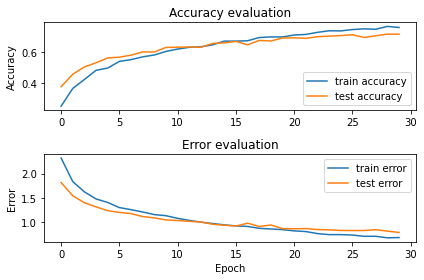
\includegraphics[width=0.45 \textwidth]{images/cnn_keras.png} 
            \caption{CNN accuracy/error evaluation}
        \end{figure}    
            
        \subsection{Training with RNN}
            \paragraph{}
            Our RNN model uses multiple layers as well. It is of sequential type. The input goes through these layers (two LSTM layers, one dense layer and one output layer). The result gets flattened out and normalized into either one of ten possible results of music genres. Once the model has been created, the test data is fitted into it. When observing testing accuracy, we obtain the following result: 59.11\%
            
        \begin{figure}[H]
            \centering
            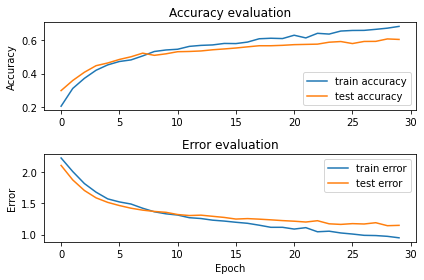
\includegraphics[width=0.45\textwidth]{images/rnn_keras.png} 
            \caption{RNN accuracy/error evaluation}
        \end{figure}